\documentclass{beamer}
\usetheme{default}

\logo{
\includegraphics[width=.3in]{logo.png} \hspace{1em} Womprats T-16}
\title{ECE411 Final Presentation}
\subtitle{Womprats T-16 Audio Synthesizer}
\author{A. Goetz \and B. Kanyid \and J. Pugh \and K. Riedl}
\institute[PSU]{
  Maseeh College of Engineering and Computer Science\\
  Portland State University\\
  Portland, Oregon 97207  
}
\date{\today}


\begin{document}
\begin{frame}[plain]
  \titlepage
\end{frame}



% 30 seconds for overview
\section{Overview} 
\frame{{Project Overview} 
  \textit{What is the T-16 Audio Synth?}
  
  \pause A flexible Audio Synthesizer platform, capable of sweet
  riffs, and catchy hooks.  }


%\frame{\titlepage}
\frame{\frametitle{Agenda}\tableofcontents} 

\subsection{Objective}
\frame{{Objective}
  \textit{What is the objective of the T-16?}
\begin{itemize}
  \pause 
  \item Make Dead Week in the Capstone Lab as annoying as possible.

  \pause
  \item Demonstrate our ``Phat Engineering Skillz''

  \pause
  \item Develop an extensible music platform.

  \pause 
  \item Develop a project that is easy to demonstrate in an interview situation. 
\end{itemize}
}

\subsection{Requirements}
\frame{{Requirements}
\begin{itemize}
\item Avoid  mechanical complexity
\item Cheap to build
\item Cheap tools
\item Use Free Tools
\item Gracefully Degradeable
\item Breadboardable
\item Demonstratable in an interview situation
\end{itemize}

}
\subsection{Approach}
\frame{{Approach}
Project Management \& Documentation tools
\begin{itemize}
\item GanttProject
\item Redmine
\item \LaTeX
\end{itemize}

Technical tools
\begin{itemize}
\item KiCad EDA
\item LPCXpresso Code Red IDE
\item Git
\end{itemize}
}

\section{Design}
\frame{\frametitle{Design}
[Design text here]\\

  \begin{figure}[htb]
    \centering
    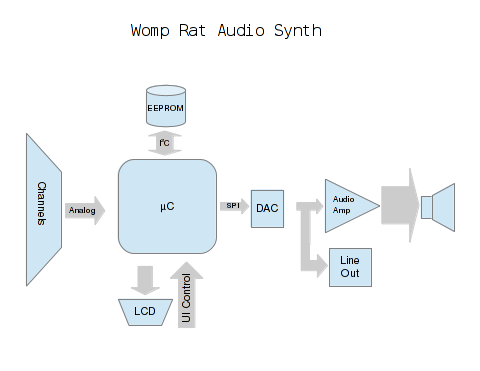
\includegraphics[width=0.7\textwidth]{BlockLevelDiagram.png} 
    \caption{Block Diagram Overview}
  \end{figure}

}

\subsection{Implementation}
\frame{{Implementation}
The parts chosen for making the audio synthesizer:
\begin{itemize}
  \pause
\item Microcontroller: NPX LPC 1114
  \pause
\item EEPROM: Atmel AT24C128C
  \pause
\item LCD: EA DOGS102W-6 +EA LED39x41-W
  \pause
\item Channels: 
  \pause
\item DAC: MCP4921
  \pause
\item Audio Amplifier: LM4875
\end{itemize}
}

\subsection{PCB Layout}
\frame{{PCB Layout} 

\begin{center}
 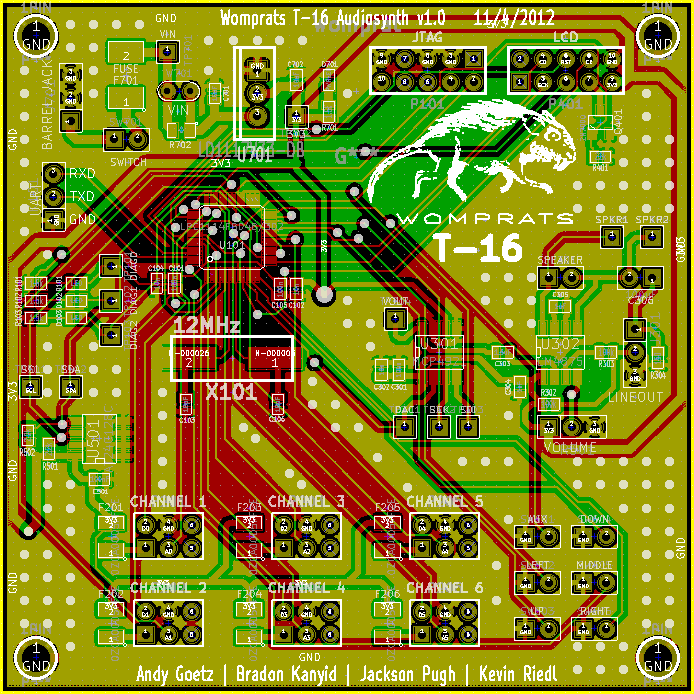
\includegraphics[width=0.7\textwidth]{pcb.png}
\end{center}
}


\begin{frame}{Lessons Learned}
\end{frame}
\subsection{Testing \& Debugging}
\frame{{Testing \& Debugging}
\begin{itemize}
  \pause
\item Microcontroller

  \begin{itemize}
    \pause
    \item Programming Test
    \pause
    \item Diagonistic Test
    \pause
    \end{itemize}
\item EEPROM
  \begin{itemize}
    \pause
    \item Read/Write Byte Test
    \pause
    \item Read/Write Burst Test
    \pause
    \end{itemize}
\item LCD
  \begin{itemize}
    \pause
    \item LCD Test
    \pause
    \item Button Test
    \pause
  \end{itemize}
\item DAC
  \begin{itemize}
    \pause
    \item I/O Test (DAC Test)
    \pause
    \end{itemize}
\item Audio Amplifier
  \begin{itemize}
    \pause
    \item Frequency Test
    \pause
    \item Line-out Test
    \pause
    \item Volume Control Test
    \pause
    \end{itemize}
\item Power Supply
  \begin{itemize}
    \pause
    \item Fuse Test
    \pause
    \item Voltage Ripple Test
    \pause
    \end{itemize}
\end{itemize}
}

\subsection{Integration Tests}
\frame{{Integration Tests}
\begin{itemize}
  \pause
  \item Power-On Self-Test
  \pause
  \item DAC-Audio Amplifier Test
  \pause
  \item Display Womprat on LCD screen
\end{itemize}
}

\subsection{Results}
\frame{{Results}
[Results text here]
}

\section{Team Evaluation}
\frame{\frametitle{Team Evaluation}
[Team Evaluation text here]
}
\subsection{Contributions}
\frame{{Contributions}
[Contributions text here]
}
\subsection{Lessons Learned}
\frame{{Lessons Learned}
  Bradon Kanyid

  Andy Goetz

  Kevin Riedl

  Jackson Pugh

}


%\section{Design Choices}
%\frame{\frametitle{Design Choices} 
%Design Choices text here
%}

%\begin{frame}{Design Choices}
%  \begin{itemize}
%    \pause
%  \item KiCad
%    \pause
%  \item LPC1114
%    \pause
%  \item GanttProject
%    \pause
%  \item \LaTeX
%    \end{itemize}
%\end{frame}



\end{document}
